\documentclass[aspectratio=1610]{beamer}

\mode<presentation>
{
  \usetheme[noheadline]{age}
}

% load languages (last language is the main language)
% select language with \selectlanguage{<language>}
\usepackage[ngerman,english]{babel}

% load fonts
\usepackage{fontspec}
\setsansfont{Open Sans} % beamerfontthemeage.sty sets all text to sans serif

% hyperlinks
\usepackage{hyperref}

% Bibliography
\usepackage[
  backend=biber,   % use modern biber backend
  autolang=hyphen, % load hyphenation rules for if language of bibentry is not german, has to be loaded with \setotherlanguages in the references.bib use langid={en} for english sources
  sorting=none,    %
  style=authoryear,% change citation style
]{biblatex}
\addbibresource{references.bib}  % the bib file to use
\DefineBibliographyStrings{american}{andothers = {{et\,al\adddot}}}  % replace u.a. with et al.

\title[Short Title]% (optional, use only with long paper titles)
{Long Presentation Title}

\subtitle
{Include An Optional Subtitle}

\author[F.~Author] % (optional, use only with lots of authors)
{\underline{First~Author}\inst{1} \and Second~Author\inst{1} \and Third~Author\inst{2} \and Fourth~Author\inst{2}}
% - Give the names in the same order as the appear in the paper.
% - Use the \inst{?} command only if the authors have different
%   affiliation.

\institute[Uni Kassel] % (optional, but mostly needed)
{
  \inst{1}%
  Institute of Physics and CINSaT\\
  University of Kassel
  \and
  \inst{2}%
  Department of Something\\
  University of Somewhere}
% - Use the \inst command only if there are several affiliations.
% - Keep it simple, no one is interested in your street address.

\date[DPG 2024] % (optional, should be abbreviation of conference name)
{DPG-Frühjahrstagung SAMOP, 2024}
% - Either use conference name or its abbreviation.
% - Not really informative to the audience, more for people (including
%   yourself) who are reading the slides online

\subject{Physics}
% This is only inserted into the PDF information catalog. Can be left
% out. 



% Add logos to the title page
\titlegraphic{%
  \begin{columns}
    \column{.3\textwidth}
    \centering
    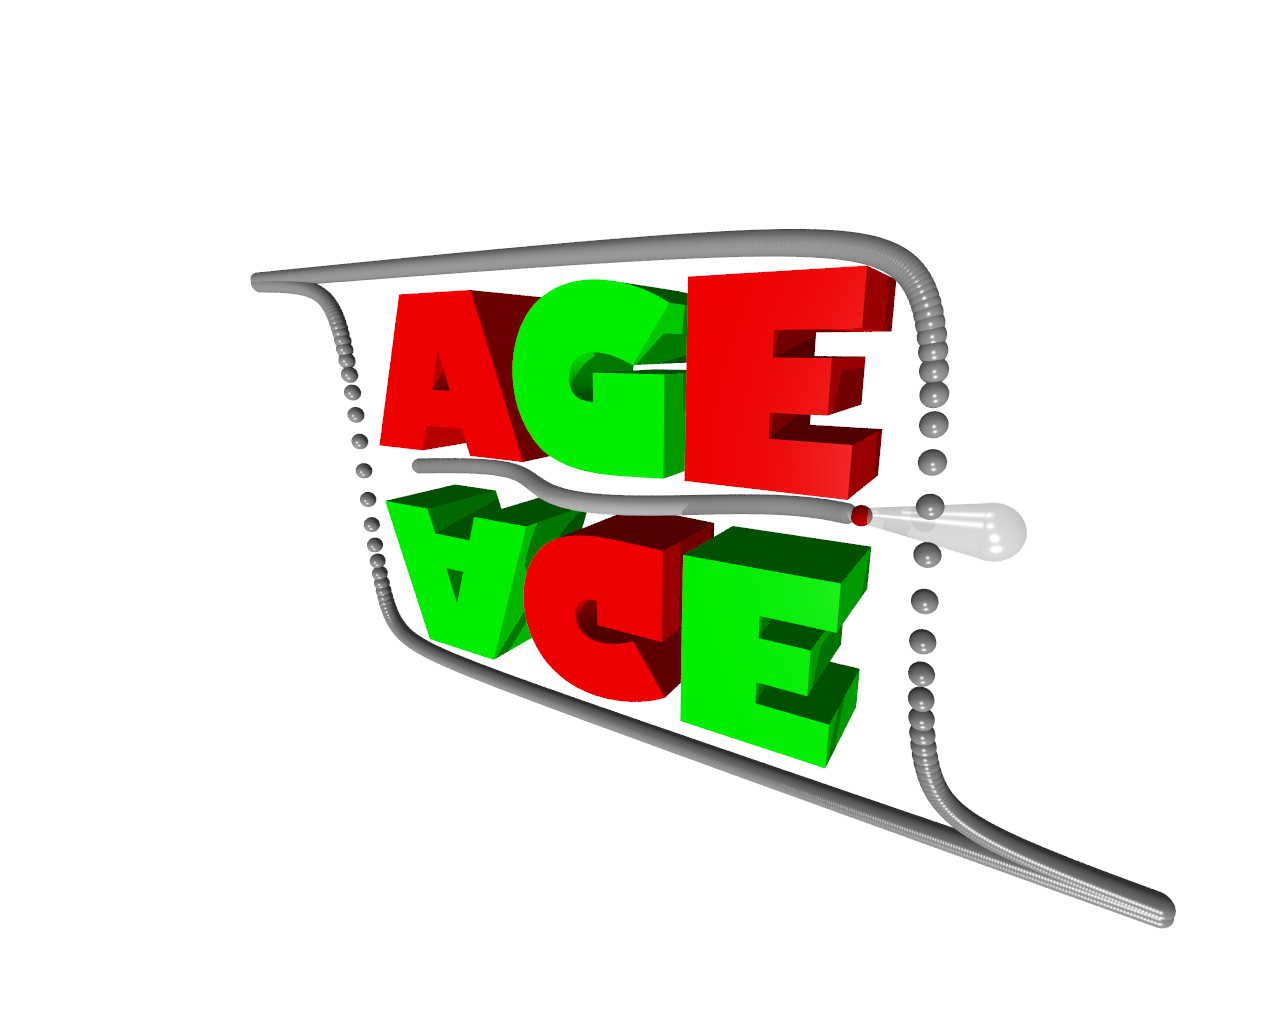
\includegraphics[height=0.2\textheight]{logos/age.png}%
    \column{.3\textwidth}
    \centering
    
\includegraphics[height=0.075\textheight]{logos/dfg.jpg}%
    \column{.4\textwidth}
    \centering
    
\includegraphics[height=0.2\textheight]{logos/hzb.png}%
  \end{columns}
}%



% Uncomment this, if you want the table of contents to pop up at
% the beginning of each subsection:
%\AtBeginSubsection[]
%{
%  \begin{frame}<beamer>{Outline}
%    \tableofcontents[currentsection,currentsubsection]
%  \end{frame}
%}


% If you wish to uncover everything in a step-wise fashion, uncomment
% the following command: 

%\beamerdefaultoverlayspecification{<+->}

\makeatletter
\newcommand{\showfont}{encoding: \f@encoding{},
  family: \f@family{},
  series: \f@series{},
  shape: \f@shape{},
  size: \f@size{}
}
\makeatother


\begin{document}

\begin{frame}
  \titlepage
\end{frame}

%\begin{frame}{Outline}
%  \tableofcontents % You might wish to add the option [pausesections]
%\end{frame}


% Structuring a talk is a difficult task and the following structure
% may not be suitable. Here are some rules that apply for this
% solution: 

% - Exactly two or three sections (other than the summary).
% - At *most* three subsections per section.
% - Talk about 30s to 2min per frame.

% - A conference audience is likely to know very little of what you
%   are going to talk about. So *simplify*!
% - In a 20min talk, getting the main ideas across is hard
%   enough. Leave out details, even if it means being less precise than
%   you think necessary.
% - If you omit details that are vital to the proof/implementation,
%   just say so once. Everybody will be happy with that.

\section{Section Title (Currently Only Visible In TOC)}

\subsection{Subsection Title (Currently Only Visible In TOC)}

\begin{frame}{Frame Title}{Frame Subtitles Currently Do Nothing}
  % - A title should summarize the slide in an understandable fashion
  %   for anyone who does not follow everything on the slide itself.
  % - Subtitles do not work with the current theme
  \begin{itemize}
    \item Use \texttt{itemize} a lot.
    \item Use very short sentences or short phrases.
  \end{itemize}
  \showfont
\end{frame}

\begin{frame}{Latex Beamer Overlays}
  You can create overlays\dots
  \begin{itemize}
    \item using the \texttt{pause} command:
    \begin{itemize}
      \item First item.
      \pause
      \item Second item.
    \end{itemize}
    \item using overlay specifications:
    \begin{itemize}
      \item<3-> First item.
      \item<4-> Second item.
    \end{itemize}
    \item using the general \texttt{uncover} command:
    \begin{itemize}
      \uncover<5->{\item First item.}
      \uncover<6->{\item Second item.}
    \end{itemize}
    \item<7-> or look at: \href{https://www.overleaf.com/learn/latex/Beamer_Presentations\%3A_A_Tutorial_for_Beginners_(Part_4)\%E2\%80\%94Overlay_Specifications}{Overleaf Overlay Tutorial for Beginners}
  \end{itemize}
\end{frame}


\begin{frame}{Blocks}
  \begin{block}{You Can Use Blocks}
    \begin{itemize}
      \item References go into the references.bib file.
      \item There are some examples [\cite{biblatex,einstein}] in there.
      \item Feel free to modify the theme to your liking.
    \end{itemize}
  \end{block}
  \begin{alertblock}{You Can Use Alertblocks}
    \begin{itemize}
      \item<alert@1> This is alerted first.
      \item<alert@2> This is alerted second.
    \end{itemize}
  \end{alertblock}
  \begin{exampleblock}{You Can Use Exampleblocks}
    \begin{itemize}
      \item This is an example.
    \end{itemize}
  \end{exampleblock}
\end{frame}


\section*{Summary}

\begin{frame}{Summary}

  % Keep the summary *very short*.
  \begin{itemize}
    \item The \alert{first main message} of your talk in one or two lines.
    \item The \alert{second main message} of your talk in one or two lines.
    \item Perhaps a \alert{third message}, but not more than that.
  \end{itemize}
  
  % The following outlook is optional.
  \vskip0pt plus.5fill
  \begin{itemize}
    \item Outlook
    \begin{itemize}
      \item Something you haven't solved.
      \item Something else you haven't solved.
    \end{itemize}
  \end{itemize}
\end{frame}


\section{Acknowledgements}

\begin{frame}{Acknowledgements}
    \begin{figure}
        \centering
        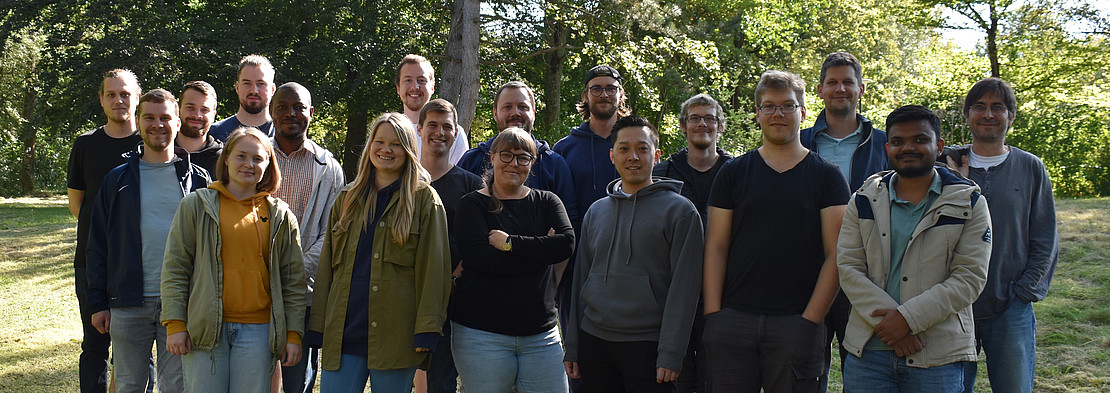
\includegraphics[width=\textwidth]{images/group_photo.jpg}
    \end{figure}
    \centering \Huge
    \emph{Thank you for your attention!}
\end{frame}


% Appendix 
\appendix
\section<presentation>*{\appendixname}
\subsection<presentation>*{References}

\begin{frame}[allowframebreaks]{References}
  \printbibliography
\end{frame}

\end{document}

